\documentclass{IEEEtran}
\usepackage[table,xcdraw]{xcolor}
\usepackage{float}
\usepackage{tikz}
\usepackage{cite}
\usepackage{graphicx}
\usepackage{pgfplots}
\usepackage{adjustbox}
\usepackage{url}

\usepackage{listings}
\usepackage{color}

\definecolor{dkgreen}{rgb}{0,0.6,0}
\definecolor{gray}{rgb}{0.5,0.5,0.5}
\definecolor{mauve}{rgb}{0.58,0,0.82}

\definecolor{bblue}{HTML}{4F81BD}
\definecolor{rred}{HTML}{C0504D}
\definecolor{ggreen}{HTML}{9BBB59}
\definecolor{ppurple}{HTML}{9F4C7C}

\lstset{frame=tb,
    language=Java,
    aboveskip=3mm,
    belowskip=3mm,
    showstringspaces=false,
    columns=flexible,
    basicstyle={\small\ttfamily},
    numbers=none,
    numberstyle=\tiny\color{gray},
    keywordstyle=\color{blue},
    commentstyle=\color{dkgreen},
    stringstyle=\color{mauve},
    breaklines=true,
    breakatwhitespace=true,
    tabsize=3,
    xleftmargin=1cm,
    xrightmargin=1cm
}
 
\title{System Management Interrupts and Their Effects}
%\author{Konstantin, Stephanie, Josef, William, Vishes, Manjeet}
\author{
    Manjeet Bhatia, William Huiras, Vishesh Jain, Konstantin Macarenco, Josef Mihalits and Stephanie Sohn\\
}

\begin{document}
\maketitle
\thispagestyle{plain}
\pagestyle{plain}
\begin{abstract}
System Management Interrupts (SMIs) are explored at a fundamental level and their effects are determined upon benchmarks, including Linux kernel compilation, NBench, MPI functions, Netperf, LMBench, and CPU power state reports. Findings reconfirm that performance degradation scales with the latency of the SMI. Additional results show that SMI effects are dampened with multi-threading and that performance degradation is additive when SMIs are enabled upon multiple communicating nodes. Lastly, it was found that SMI’s continue to significantly affect power consumption and CPU sleep states.
\end{abstract}

\tableofcontents
\section{Introduction}\label{sec:intro}
A System Management Interrupt (SMI) is a method of entry into System Management Mode (SMM). System Management Mode is a mode that is more privileged than operating systems and hypervisors. SMIs pre-empt the operations of the operating system or hypervisor causing all processor cores to stop and enter SMM. Additionally, such preemption is invisible to these systems. Thus, SMIs not only take time away from the operating system or hypervisor, but they unpredictably interrupt them as well.\\
\indent There exist several reasons for the existence of SMM. Originally, SMM was created to allow events specific to the machinery to be properly maintained, including power throttling, hardware emulation, and system health checks. More recently, with security compromises of hypervisors, such as Xen, SMM has been leveraged as a platform to detect malicious code injection into hypervisors, such as RIMM (Runtime Integrity Measurement Mechanisms). RIMM is able to periodically check the hypervisor code for changes by entering SMM. The use of SMM is advantageous as it lies in an unaccesible address space untouchable by malware. Nevertheless, the amount of time needed to reside in SMM in order to perform security checks is prohibitively disruptive to the normal functioning of programs in the level of the hypervisor and operating system.\\
\indent Previous studies have been performed to determine the effects of SMIs \cite{KD}. These studies of SMI effects include: the measurement of scheduler tick intervals with differing SMI latencies, the measurement of percent time in C-states, audio and video driver disruption, OpenSSL and time accounting (for billing purposes), and effects upon the hypervisor Xen, including benchmarks such as Linux compilation time, TCP networking, disk reads, and compute-intensive encryption. From these experiments, it is concluded that while shorter length SMIs produce jitter, their effects upon performance are not drastically debilitating. On the other hand, long SMIs (100 ms or greater) are detrimental to performance, increasing the run times of programs, and SMIs are shown to increase energy usage, cause time scaling discrepancies, reduce throughput, and produce audio and video distortions.\\
\indent We aim to both verify select experiments above, as well as to add to them. The remainder of the paper includes further experiments in the areas of fundamental SMI studies, and the effects of SMIs upon various benchmarks including: CPU bound benchmarks and Linux compilation, MPI (Message Passing Interface) routines, Netperf, LMBench, NBench, and Turbostat.

\section{Testing}\label{sec:testing}
\subsection{Hardware and Software}\label{sub:hardware_and_software}
Eight machines were used for experiments with the naming convention in the form of smitestN, where N is the number of a node in the range 2-8 (e.g. smitest2, smitest3, and so on); the first node was named ``smitest''. An additional external server ``wyeasthead'' was used for time synchronization experiments. All the nodes have the following configurations: Intel(R) Xeon(R) CPU E5520  @ 2.27GHz, cache size of 8192 KB, and 12Gb RAM. Hyperthreading was disabled on all nodes except for smitest3. Gigabit ethernet devices included Ethernet controller Intel Corporation 82567LM Gigabit Network Connection and Broadcom Corporation NetXtreme II BCM5716 Gigabit Ethernet. For software, all machines ran on CentOS 5.10, kernel version 3.0.4.

\subsection{SMI Driver}\label{sub:smi_driver}
Driver software was written to create SMIs. It operates to produce two types of SMIs, named ``short'' and ``long'', with latencies of 1-3 ms and 100-110 ms, respectively. The driver also was coded to possess features to:
\begin{itemize}
  \item Measure SMI latency in TSC (time stamp counter)
  \item Start/Stop recurring SMIs
  \item Count the number of SMIs that occurred using an elapsed TSC count
\end{itemize}

\subsection{SMI Length Investigation}\label{sub:km_smilength}

\textbf{Background}
The SMI driver uses the TSC counter to measure the average SMI latency, yet we came to conclusion that this approach is not accurate enough due to TSC limitations. TSC on tested systems increases at the constant rate $R=CPU\_top\_speed$, and it reflects only the time passed between two reads, which might be affected by preemption. Thus, experiments were created to measure SMI length.

\textbf{Methodology}
The driver schedules an SMI at the rate $x$, i.e. one SMI is triggered every $x$ jiffies. In $x86\_64$ systems, one jiffy lasts one millisecond, so the driver triggers one SMI every $x$ $ms$. If the SMI length and schedule interval equal exactly one second, then after $N$ seconds the difference between elapsed time $N$ and number of occurring SMIs will equal zero.\\
Let $x$ be driver rate in $ms$, $l$ be the SMI length in $ms$, $N$ be the elapsed time in seconds, and $C$ be the amount of SMIs that occurred, then:\\
\begin{eqnarray}
  D = N-C\times\frac{(x+l)}{1000}
\end{eqnarray}
   equals zero, if 
\begin{eqnarray}
   x+l=1 sec
\end{eqnarray}
SMI length tests were performed on each machine for schedule interval $x$ starting at one SMI for every $880$ ms for long SMIs, and one SMI for every $990$ ms for short SMIs, and ending at one SMI for every $1000$ ms. Tests were performed for $N=500$ seconds for long SMIs, and $N=1000$ seconds for short SMIs. SMI length, $l$, ranged from $1$ - $3$ $ms$ for short SMIs. Pseudo-code to perform this is shown below. The algorithm was implemented as a bash script, because the load/unload kernel module is required to change driver rate.

\begin{figure}[H]
\begin{lstlisting}
#define x 880
set_driver_rate x
start_recurring_smis
// Get smicount: echo 6 >
/proc/smidriver
get_current_smi_count start_smi_c
wait N seconds
get_current_smi_count end_smi_c
save x and (start_smi_c - end_smi_c)
\end{lstlisting}
\caption{Pseudo code for SMI length algorithm}
\label{mk_smilengthpseudo}
\end{figure}

The algorithm was implemented as a bash script, because load/unload kernel module is required to change driver rate.

\textbf{Results and Discussion}
Results of SMI rate studies are shown in Figures ~\ref{km_smilength_short} and ~\ref{km_smilength_long}. On the graphs it can be seen that there is zero deviation in the range of $x=997$ - $999$ (scheduling of $1$ SMI per every ~998 ms) for short SMIs and in the range of $x=890$ - $895$ for long SMIs. Therefore interrupt length, $l$, being $1000-x$, allows us to determine that the accurate short SMI length is $1$ - $3$ ms and that the long SMI length is $110$ - $105$ ms. The only anomaly occurs for the case of smitest3 where, deviation equals zero in the range $x=960$ - $965$ for long SMIs. This yields the length of $40$ to $35$ ms. We assume that this is caused by hyperthreading, since SMM code runs in parallel and finishes faster.

\begin{figure}[h]
  \centering
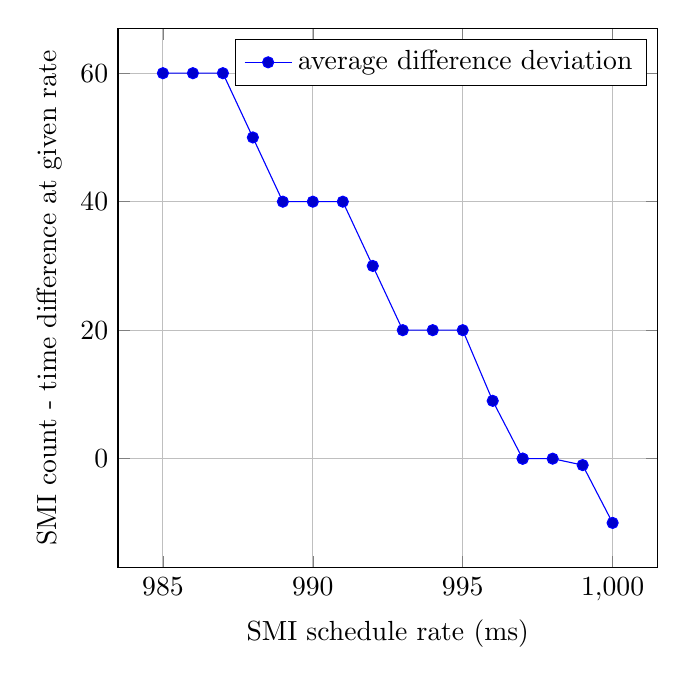
\begin{tikzpicture}
\begin{axis}[
height=240pt,
width=240pt,
grid=major,
xlabel={SMI schedule rate (ms)},
ylabel={SMI count - time difference at given rate}
]

%\addplot {-x^5 - 242};
%\addlegendentry{model}
\addplot coordinates {
(985,60) (986,60) (987,60) (988,50) (989,40) (990,40) (991,40) (992,30) (993,20) (994,20) (995,20) (996,9) (997,0)
(997,0) (998,0) (999,-1)
(1000,-10)
};\label{p4}
%\addplot coordinates {
%(999,-1) (1000,-10)
%};
%\addplot coordinates {
%(997,0) (998,0) (999,-1)
%};
\addlegendentry{average difference deviation}
\end{axis}
\end{tikzpicture}
\caption[Caption in ToC]{Short SMIs length difference deviation at SMI rate. 0 deviation occurs when smilength + rate = 1sec }
\label{km_smilength_short}
\end{figure}

\begin{figure}[h]
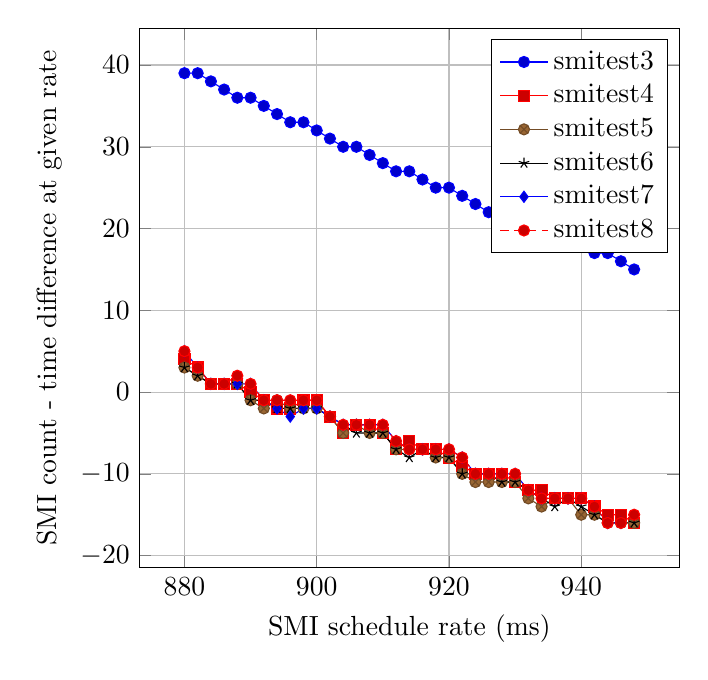
\begin{tikzpicture}
\begin{axis}[
height=240pt,
width=240pt,
grid=major,
xlabel={SMI schedule rate (ms)},
ylabel={SMI count - time difference at given rate}
]

%\addplot {-x^5 - 242};
%\addlegendentry{model}
\addplot coordinates {
(880,39) (882,39) (884,38) (886,37) (888,36) (890,36) (892,35) (894,34) (896,33) (898,33) (900,32) (902,31) (904,30) (906,30) (908,29) (910,28) (912,27) (914,27) (916,26) (918,25) (920,25) (922,24) (924,23) (926,22) (928,22) (930,21) (932,21) (934,19) (936,19) (938,18) (940,18) (942,17) (944,17) (946,16) (948,15) 
};\label{p4}
\addplot coordinates {
(880,4) (882,3) (884,1) (886,1) (888,1) (890,0) (892,-1) (894,-2) (896,-2) (898,-1) (900,-1) (902,-3) (904,-5) (906,-4) (908,-4) (910,-5) (912,-7) (914,-6) (916,-7) (918,-7) (920,-8) (922,-9) (924,-10) (926,-10) (928,-10) (930,-11) (932,-12) (934,-12) (936,-13) (938,-13) (940,-13) (942,-14) (944,-15) (946,-15) (948,-16) 
};\label{p5}
\addplot coordinates {
(880,3) (882,2) (884,1) (886,1) (888,1) (890,-1) (892,-2) (894,-1) (896,-2) (898,-2) (900,-2) (902,-3) (904,-5) (906,-4) (908,-5) (910,-5) (912,-7) (914,-7) (916,-7) (918,-8) (920,-8) (922,-10) (924,-11) (926,-11) (928,-11) (930,-11) (932,-13) (934,-14) (936,-13) (938,-13) (940,-15) (942,-15) (944,-16) (946,-16) (948,-16) 
};\label{p5}
\addplot coordinates {
(880,3) (882,2) (884,1) (886,1) (888,1) (890,-1) (892,-1) (894,-2) (896,-2) (898,-2) (900,-2) (902,-3) (904,-4) (906,-5) (908,-5) (910,-5) (912,-7) (914,-8) (916,-7) (918,-8) (920,-8) (922,-10) (924,-10) (926,-10) (928,-11) (930,-11) (932,-12) (934,-13) (936,-14) (938,-13) (940,-14) (942,-15) (944,-16) (946,-16) (948,-16) 
};\label{p5}
\addplot coordinates {
(880,5) (882,3) (884,1) (886,1) (888,1) (890,1) (892,-1) (894,-2) (896,-3) (898,-2) (900,-2) (902,-3) (904,-4) (906,-4) (908,-4) (910,-4) (912,-6) (914,-7) (916,-7) (918,-7) (920,-7) (922,-8) (924,-10) (926,-10) (928,-10) (930,-10) (932,-12) (934,-13) (936,-13) (938,-13) (940,-13) (942,-14) (944,-16) (946,-16) 
};\label{p5}
\addplot coordinates {
(880,5) (882,3) (884,1) (886,1) (888,2) (890,1) (892,-1) (894,-1) (896,-1) (898,-1) (900,-1) (902,-3) (904,-4) (906,-4) (908,-4) (910,-4) (912,-6) (914,-7) (916,-7) (918,-7) (920,-7) (922,-8) (924,-10) (926,-10) (928,-10) (930,-10) (932,-12) (934,-13) (936,-13) (938,-13) (940,-13) (942,-14) (944,-16) (946,-16) (948,-15) 
};\label{p5}
\addlegendentry{smitest3}
\addlegendentry{smitest4}
\addlegendentry{smitest5}
\addlegendentry{smitest6}
\addlegendentry{smitest7}
\addlegendentry{smitest8}
\end{axis}
\end{tikzpicture}
\caption[Caption in ToC]{Long SMIs length difference deviation at SMI rate. 0 deviation occurs when smilength + rate = 1sec }
\label{km_smilength_long}
%\caption[Caption in ToC]{Short SMI's length deviation to SMI rate. Zero deviation occurs when SMI length + rate = 1 sec }
%\end{figure}
%
%\begin{figure}[h]
%  \centering
\end{figure}
\textbf{Conclusion and Future Work}
The above presented technique to measure SMI latency is more accurate than the method of simply reading the $TSC$ counter. It is especially noticeable on a machine with enabled hyperthreading, where the $TSC$ counter fails to notice the difference. In average it is 40\% more accurate on machines with no hyperthreading enabled, and it is 110\% better on a machine with hyperthreading enabled. The main disadvantage of this type of new testing is that it requires a significant amount of time to perform. In the future, it would be interesting to enable hyperthreading on more machines, and investigate in depth how hyperthreading affects SMIs.

\subsection{System Time Delay}\label{sub:km_system_time}
\textbf{Background}
While performing the SMI length investigation, peculiar wall times were noticed on all the test machines except the gateway machine. Below is a snapshot of all systems' wall time.

\begin{figure}[t]
\begin{lstlisting}
June 6 18:46:50 smitest
June 6 19:45:09 smitest2
June 6 18:54:42 smitest3
June 6 16:26:14 smitest4
June 6 17:43:26 smitest5
June 6 18:37:45 smitest6
June 6 13:12:27 smitest7
June 6 13:00:57 smitest8
June 6 18:44:44 wyeasthead - gateway (real time).
\end{lstlisting}
\caption[Wall time snapshot]{Wall time snapshot}
\label{km_timesnapshot}
\end{figure}

This difference in wall clock times could be a coincidence caused by uncoordinated system setup, or it could have been produced by repeated testing, where recurring SMIs, especially long ones, would affect the system's wall time. To investigate if this was indeed the case further timing tests were executed on smitest and smitest6. The time difference was obtained by checking with the machine $wyeasthead$. $wyeasthead$ was chosen for this purpose because it is a gateway machine that has Internet access and thus its current time is correct. Additionally, no SMIs are invoked upon this machine, so its wall time is not affected.

\textbf{Methodology}
For every $N$ SMIs invoked, the time difference via the gateway was obtained. Time differences were taken every $N=1000$ SMIs. Graphs were plotted in the following way: the $X$-axis is the number of SMIs that have occurred, and the $Y$-axis is the time difference between test and gateway machines. Tests were performed for long SMIs only, due to the assumption that short SMIs do not drastically affect the system clocks.

\textbf{Results and Discussion}
Figure~\ref{km_timedelay1} displays results for two consecutive runs where the blue plot represents one run and the red plot represents another. In this figure, wyeasthead is running behind smitest3 (the difference is about 2 min), and as time passes, the difference decreases, i.e. time at smitest approaches the time at wyeasthead. The graph of Figure~\ref{km_timedelay2} is the same test (a single run only) but ran on smitest6. In this case, wyeasthead time is ahead, so the difference in time is widening overtime.
\begin{figure}[h]
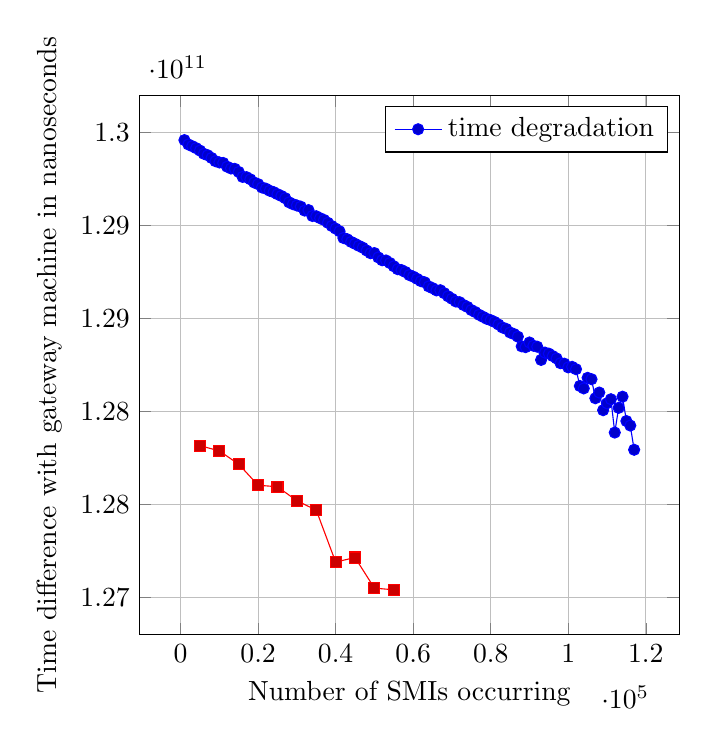
\begin{tikzpicture}
\begin{axis}[
height=240pt,
width=240pt,
grid=major,
xlabel={Number of SMIs occurring},
ylabel={Time difference with gateway machine in nanoseconds}
]
%\addplot {-x^5 - 242};
%\addlegendentry{model}
\addplot coordinates {
(1000,129459799459) (2000,129436547164) (3000,129427275322) (4000,129416736398) (5000,129403479114) (6000,129386243455) (7000,129378292604) (8000,129363799006) (9000,129346425702) (10000,129339474525) (11000,129336744680) (12000,129316826017) (13000,129307091482) (14000,129304951063) (15000,129288422843) (16000,129261810844) (17000,129260313403) (18000,129248841852) (19000,129231561282) (20000,129222935927) (21000,129204898277) (22000,129198358280) (23000,129187230124) (24000,129179879789) (25000,129168716813) (26000,129159161189) (27000,129147254027) (28000,129124932156) (29000,129114990065) (30000,129107970610) (31000,129101456992) (32000,129080475599) (33000,129082959845) (34000,129051417764) (35000,129049889510) (36000,129039395377) (37000,129030168940) (38000,129014812308) (39000,128997628058) (40000,128983510063) (41000,128969230257) (42000,128933256049) (43000,128926092923) (44000,128911948959) (45000,128901788487) (46000,128890773980) (47000,128880826120) (48000,128865515906) (49000,128850996690) (50000,128851566479) (51000,128828380985) (52000,128813153821) (53000,128811858605) (54000,128798247871) (55000,128780831788) (56000,128765049954) (57000,128760009196) (58000,128749834869) (59000,128733608412) (60000,128725155845) (61000,128713359822) (62000,128700628020) (63000,128694096812) (64000,128672350837) (65000,128663016906) (66000,128650993811) (67000,128651829633) (68000,128636039533) (69000,128619083894) (70000,128605868825) (71000,128591244615) (72000,128587031779) (73000,128572166987) (74000,128561962818) (75000,128545070474) (76000,128534453684) (77000,128519632349) (78000,128508810860) (79000,128497767617) (80000,128490441352) (81000,128481054219) (82000,128467276774) (83000,128451475560) (84000,128443597797) (85000,128424316590) (86000,128416062036) (87000,128401913250) (88000,128349669580) (89000,128345414940) (90000,128370563755) (91000,128353156495) (92000,128347834575) (93000,128276662913) (94000,128315896219) (95000,128310451362) (96000,128297284845) (97000,128284642030) (98000,128259022910) (99000,128256350368) (100000,128236586805) (101000,128239278756) (102000,128226790154) (103000,128136337450) (104000,128123355436) (105000,128180159892) (106000,128172922695) (107000,128070390283) (108000,128101012405) (109000,128006079776) (110000,128043109312) (111000,128065044661) (112000,127885652853) (113000,128018632058) (114000,128078657151) (115000,127947640004) (116000,127923419287) (117000,127793018175) 

};\label{p4}
\addplot coordinates {
(5000,127815043448) (10000,127786985925) (15000,127715259224) (20000,127602141609) (25000,127593885743) (30000,127518551798) (35000,127468127377) (40000,127188743288) (45000,127212957014) (50000,127048352180) (55000,127039324707)

};\label{p5}
\addlegendentry{time degradation}
\end{axis}
\end{tikzpicture}
\caption[Caption in ToC]{Time delay: difference between smiteset and wyeasthead gets shorter overtime, since smitest is running ahead}
\label{km_timedelay1}
\end{figure}

\begin{figure}[h]
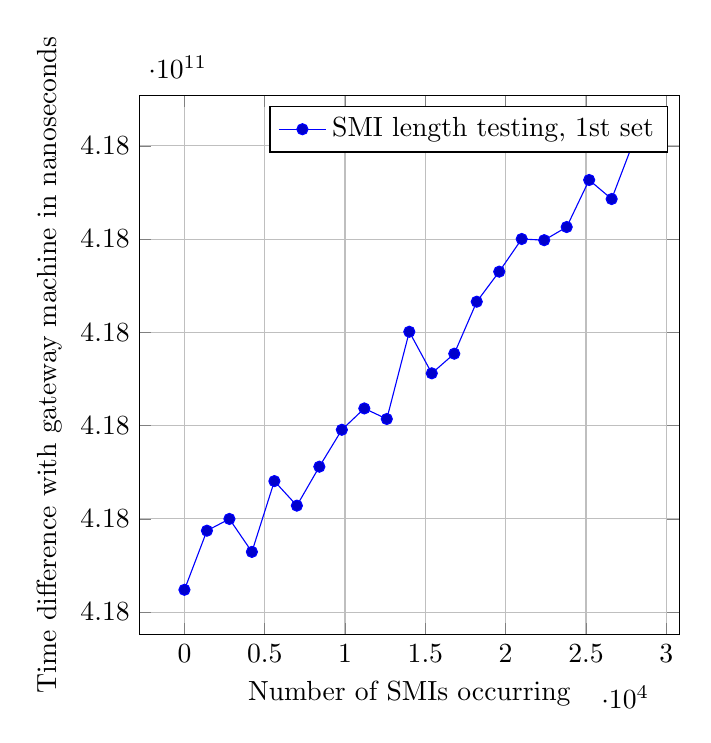
\begin{tikzpicture}
\begin{axis}[
height=240pt,
width=240pt,
grid=major,
xlabel={Number of SMIs occurring},
ylabel={Time difference with gateway machine in nanoseconds}
]

\addplot coordinates {
(0,418344774422) (1400,418357452452) (2800,418359973517) (4200,418352903608) (5600,418368087763) (7000,418362825502) (8400,418371175144) (9800,418379097365) (11200,418383673309) (12600,418381409646) (14000,418400122583) (15400,418391205090) (16800,418395413321) (18200,418406567751) (19600,418413011612) (21000,418420015697) (22400,418419759372) (23800,418422580932) (25200,418432670955) (26600,418428589668) (28000,418441227093)
};\label{p6}
\addlegendentry{SMI length testing, 1st set}
\addlegendentry{SMI length testing, 2nd set}
\end{axis}
\end{tikzpicture}
\caption[Caption in ToC]{Time delay: difference increases overtime since Smitest6 is behind wyeasthead}
\label{km_timedelay2}
\end{figure}
\textbf{Conclusion and Future work}
The system time gets delayed a time amount corresponding to the SMI length. For this reason, the delay is not noticeable at at first, nevertheless it is accumulative. This can potentially lead to a variety of synchronization problems. Interesting future studies could include performing the same test for different ranges of SMI lengths, to see the degree at which the system is affected.

\subsection{Linux Compilation and NBench}\label{sub:km_performance}

\textbf{Background}
Timed Linux compilation is a well known way to test the overall performance of a system. It represents a workload that is common for software development, and it is computationally, memory, and I/O intense. NBench is a benchmark that was created in mid 90's and consists of following tests:\\

\begin{itemize}
  \item Numeric sort - Sorts an array of long integers.
  \item String sort - Sorts an array of strings of arbitrary length.
  \item Bitfield - Executes a variety of bit manipulation functions.
  \item Emulated floating-point - A small software floating-point package.
  \item Fourier coefficients - A numerical analysis routine for calculating series approximations of waveforms.
  \item Assignment algorithm - A well-known task allocation algorithm.
  \item Huffman compression - A well-known text and graphics compression algorithm.
  \item IDEA encryption - A relatively new block cipher algorithm.
  \item Neural Net - A small but functional back-propagation network simulator.
  \item LU Decomposition - A robust algorithm for solving linear equations.
\end{itemize}

This particular benchmark was chosen due to the lack of super-user privileges on the server installation. It does not have any extra dependencies and is compatible with almost any version of Linux. The main disadvantage of NBench is that it was not designed for multicore computers. To simulate multicore behavior $n$ instances of NBench were executed at the same time, where $n$ is a number of available cores.

\textbf{Methodology}
All benchmarks were tested in three modes: No SMI, Short SMIs (one per second), Long SMIs (one per second). Twenty trials were ran for each mode and averaged. In single core tests, each instance of Linux compilation and NBench was timed using the Bash $date$ function which has fine granularity (nanoseconds). To allow for multicore tests, the Linux make file can be executed with option -j n, where n is the number of available cores. Linux compilation multi-core performance was measured the same way as for single core (using Bash $date$).\\
\indent As mention before, NBench has no native support for multicore, so to simulate multicore, $n$ instances of NBench were forked at the same time, then the main script waited until all $n$ instances completed. This was repeated 20 times. This procedure works because of load-balancing, i.e. the load is spread among all cores, therefore if $n \le c$, where $c$ is number of cores, then no more than one job is assigned to one core. Throughput is calculated as below:\\
\begin{eqnarray}
Throughput\_aver=\frac{time\_to\_complete}{number\_of\_cores}
\end{eqnarray}
Where $number\_of\_cores$ is equal to number of NBench instances, and $time\_to\_complete$ is time for single run, in which all instances of NBench finish.\\

\textbf{Results and Discussion}
%,~\ref{km_4core},~\ref{km_ht} . Short SMIs seems not to affect performance, and these tests sometimes exceed in performance to that of ones with NoSMI. This is assumed to be a standard deviation that depends on current CPU load.\\
\indent Recurring long SMIs have noticeable effects on system performance. In single core tests, they slow down performance by 10-12\% approximately Figure~\ref{fig:km_single}. In cores with hyperthreading disabled, performance suffers the most, with 75\% degradation for NBench and 65\% degradation for Linux compilation benchmark Figure~\ref{fig:km_4core}. Hyperthreading softens the problem; Linux compilation performance degradation is only 12\%, but NBench degradation is still 75\% Figure~\ref{fig:km_ht}. This can be explained by: (1) Long SMIs runs complete twice as fast consuming less CPU time, (2) Linux compilation might be able to execute more jobs with hyperthreading on, increasing performance (although it is not the same as having 8 cores) (3) NBench is not meant for multicore, therefore it cannot take advantage of hyperthreading.

\begin{figure}[h]
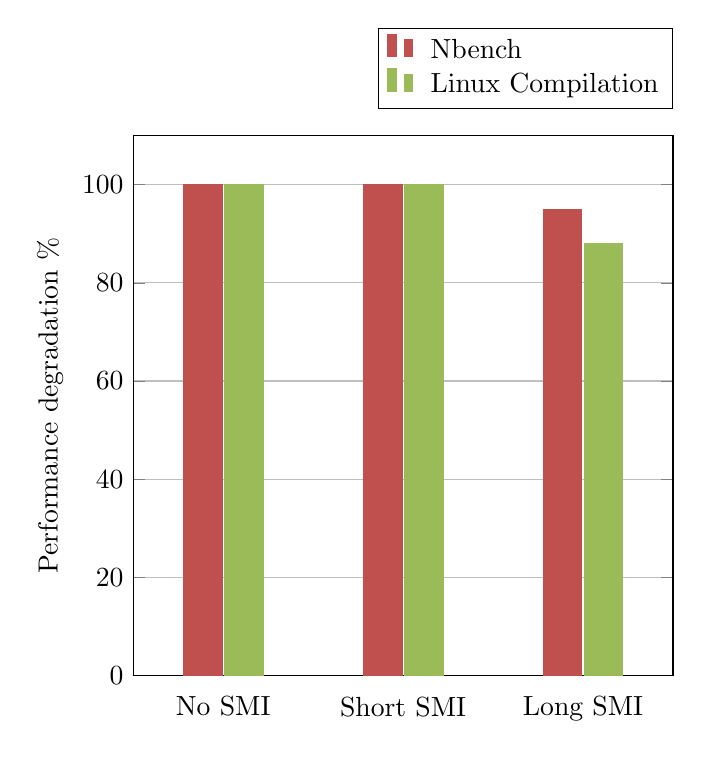
\begin{tikzpicture}
\begin{axis}[
width= 240pt,
height = 240pt,
major x tick style = transparent,
ybar=2*\pgflinewidth,
bar width=14pt,
ymajorgrids = true,
ylabel = {Performance degradation \%},
symbolic x coords={No SMI,Short SMI,Long SMI},
xtick = data,
scaled y ticks = false,
enlarge x limits=0.25,
ymin=0,
legend cell align=left,
legend style={
at={(1,1.05)},
anchor=south east,
column sep=1ex
}
]
%\addplot[style={bblue,fill=bblue,mark=none}]
%coordinates {(NoSmi, 100.0) (ShortSmi,100) (LongSmi,100.0)};

\addplot[style={rred,fill=rred,mark=none}]
 coordinates {(No SMI,100.0) (Short SMI,99.95) (Long SMI,95)};

 \addplot[style={ggreen,fill=ggreen,mark=none}]
coordinates {(No SMI,100) (Short SMI,99.95) (Long SMI,88)};

%\addplot[style={ppurple,fill=ppurple,mark=none}]
% coordinates {(NoSmi,0.74) (ShortSmi,1.07) (LongSmi,1.23)};

 \legend{ Nbench, Linux Compilation}
 \end{axis}
 \end{tikzpicture}
\caption{Single thread performance}
\label{fig:km_single}
\end{figure}

\begin{figure}[h]
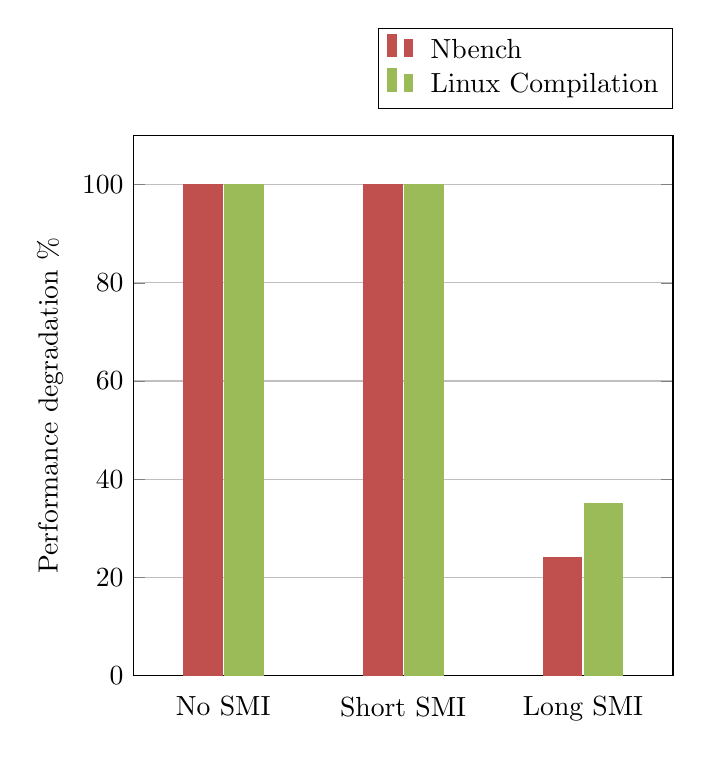
\begin{tikzpicture}
\begin{axis}[
%width= 0.85*\textwidth,
width= 240pt,
height = 240pt,
major x tick style = transparent,
ybar=2*\pgflinewidth,
bar width=14pt,
ymajorgrids = true,
ylabel = {Performance degradation \%},
symbolic x coords={No SMI, Short SMI, Long SMI},
xtick = data,
scaled y ticks = false,
enlarge x limits=0.25,
ymin=0,
legend cell align=left,
legend style={
at={(1,1.05)},
anchor=south east,
column sep=1ex
}
]
\addplot[style={rred,fill=rred,mark=none}]
 coordinates {(No SMI,100.0) (Short SMI,99.95) (Long SMI,24)};

 \addplot[style={ggreen,fill=ggreen,mark=none}]
coordinates {(No SMI,100) (Short SMI,99.95) (Long SMI,35)};

 \legend{Nbench, Linux Compilation}
 \end{axis}
 \end{tikzpicture}
\caption{Four cores, hyperthreading off}
\label{fig:km_4core}
\end{figure}

\begin{figure}[h]
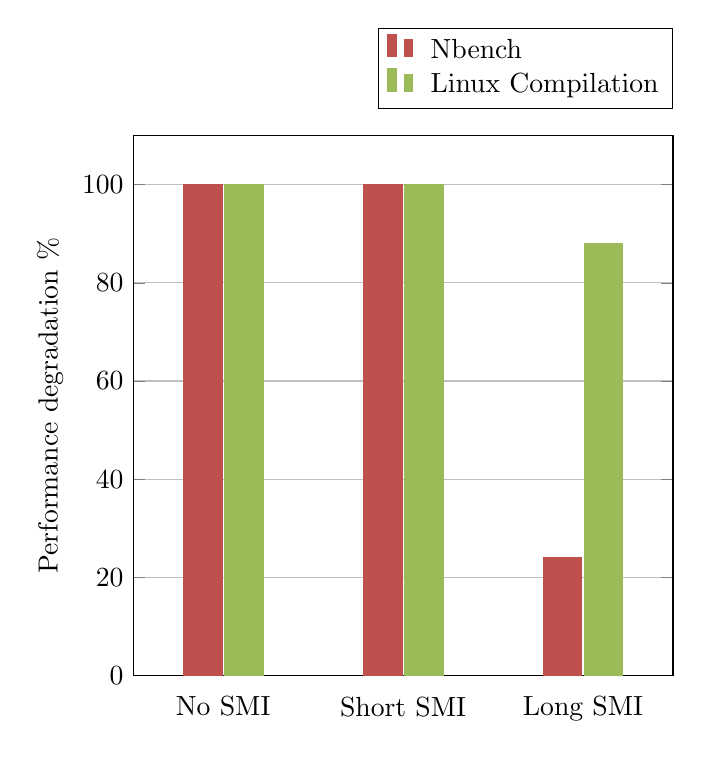
\begin{tikzpicture}
\begin{axis}[
width= 240pt,
height = 240pt,
major x tick style = transparent,
ybar=2*\pgflinewidth,
bar width=14pt,
ymajorgrids = true,
ylabel = {Performance degradation \%},
symbolic x coords={No SMI,Short SMI,Long SMI},
xtick = data,
scaled y ticks = false,
enlarge x limits=0.25,
ymin=0,
legend cell align=left,
legend style={
at={(1,1.05)},
anchor=south east,
column sep=1ex
}
]
%\addplot[style={bblue,fill=bblue,mark=none}]
%coordinates {(NoSmi, 100.0) (ShortSmi,100) (LongSmi,100.0)};

\addplot[style={rred,fill=rred,mark=none}]
 coordinates {(No SMI,100.0) (Short SMI,99.95) (Long SMI,24)};

 \addplot[style={ggreen,fill=ggreen,mark=none}]
coordinates {(No SMI,100) (Short SMI, 99.95) (Long SMI,88)};

%\addplot[style={ppurple,fill=ppurple,mark=none}]
% coordinates {(NoSmi,0.74) (ShortSmi,1.07) (LongSmi,1.23)};

 \legend{Nbench, Linux Compilation}
\end{axis}
\end{tikzpicture}
\caption{four cores with hyperthreading on}
\label{fig:km_ht}
\end{figure}

\textbf{Conclusion and Future work}
There is a large difference in performance that depends upon SMI latency, so all possible ranges of SMI length should be tested to see when noticeable performance degradation begins. This can be an outline for manufacturers and industry to help determine at which point the expansion of SMI indirect use needs to be limited.\\


\subsection{MPI}
\textbf{Background}
Message Passing Interface (MPI) is a standardized and portable message-passing system that functions on a wide variety of parallel computers. The standard of MPI provides the syntax and semantics of a core of library routines that allows for the writing of portable message-passing programs in Fortran or the C programming language \emph{\cite{WK1}}.

The MPI library contains many useful routines that establish the means of communication between parallel computers \emph{\cite{MPICH}} . Two of the most basic routines are $MPI\_Send$, which sends data in a buffer of an indicated size using a blocking mechanism to a specific node, and $MPI\_Recv$, which receives a message in a buffer of an indicated size in a blocking manner from a specific node. Other message passing routines can build upon basic send and receive patterns, including routines such as $MPI\_Allreduce$, which combines values from all processes and distributes the result back to all processes, or $MPI\_Alltoall$, which sends data of an array to the correlating numbered node, i.e. data of array index 0 goes to node 0, index 1 to node 1 and so forth; in return, the calling node will receive array data correlating to its node number. Another routine, $MPI\_Barrier$, does not send data, but it is used to synchronize processes of nodes sharing the same global communicator; it causes blocks until all processes in the communicator have reached this routine. 

MPI is interesting to examine in the presence of SMIs to determine the effects of the SMIs upon synchronization of parallel communicating computers. With SMIs enabled upon one or more computers in a cluster, it is likely that delays in one computer will exacerbate delays in all other communicating nodes. Using the above mentioned MPI routines, the effects of SMIs are examined to determine their overall implications upon cluster communication.

\textbf{Methodology}
Benchmarks were created to examine the effects of SMIs and SMI duration upon MPI routines. The particular routines of interest that were examined included: $MPI\_Send$, $MPI\_Recv$, $MPI\_Barrier$, $MPI\_Allreduce$, and $MPI\_Alltoall$. The latter three were repeatedly called in a loop for either 1,000 iterations or for 1,000,000 iterations. The former two were encoded in a ring program, passing an integer, that is incremented by each node, from one node to the next based upon the rank of the node. The highest ranked node completes the ring by passing the incremented integer back to the lowest ranked node. The entirety of this ring routine was placed in a loop, akin to the aforementioned MPI routines, with iterations of 1,000 or 1,000,000. These benchmarks were tested upon 2, 4 or 8 machines, or upon 1 machine but with 2, 4 or 8 processes communicating upon this one machine. Using the provided driver to enable SMIs, times of each benchmark were collected with no SMIs, with “short” SMIs enabled (1 SMI per second, ~0.05 ms duration of a short SMI), or with “long” SMIs enabled (1 SMI per second, 100-110 ms). The computer “smitest3” was used to launch MPI runs with indicated parameters of the number of machines, which machines, and which executable (“Ring”, “Barrier”, “AllReduce”, or “AlltoAll”). Different versions of the executables were made to indicate the number of iterations (1,000 or 1,000,000). For tests with 2 nodes, smitest3 and smitest4 were used; for 4 nodes, smitest3, smitest4, smitest5 and smitest6 were used; for 8 nodes, all 8 machines were used. For all runs in Table~\ref{ss_table1}, the Linux function “date” with option for output of time in nanoseconds was used to determine the run time of the benchmark. These runs were an average of 3 trials. For runs in Table~\ref{ss_table2}, the Linux function “time” was used, and SMI counts, as an option provided by the driver, were collected; these runs were an average of 5-8 trials; runs with high time variance were excluded from averages. To enable SMIs for Figure~\ref{ss_graph3}, each smitest machine was enabled in turn, sequentially and manually, using the driver options.

\textbf{Results and Discussion}
Benchmarks were measured to acquire runtimes. Results are shown in Table~\ref{ss_table1}. Figure~\ref{ss_graph1} displays run times for MPI benchmarks ran on 2, 4, or 8 nodes with SMIs enabled on smitest3 only, and MPI routines are encoded to repeat for 1,000 iterations. Run times last around 0.2 to 0.4 seconds. The “Ring” benchmark runs the longest (~0.10 seconds more) compared to the other benchmarks (Barrier, AllReduce, and AlltoAll). Nevertheless, similar results for normalized times occur for all the benchmarks (normalization calculation is time with no SMIs enabled divided by time with SMIs enabled multiplied by 100). Short SMI times shows on average no or little degradation, normalizing to 99\%. Curiously, some short SMI runs show faster run times than those with no SMIs enabled; for this table the highest normalization being 107\%. When comparing long SMI runs to no SMI runs, the average normalization is 90\%, matching the latency of the long SMI, which is programmed to interrupt for 1/10 of the time. No outstanding trends are noticed when comparing between MPI routine types or number of nodes (2, 4 or 8) involved in the MPI communication.

Figure~\ref{ss_graph2} displays run times for MPI benchmarks ran on 2, 4, or 8 nodes with SMIs enabled on smitest3 only, and MPI routines are encoded to repeat for 1,000,000 iterations. Iterations were increased in an attempt to reduce variance. Run times last around 75 to 300 seconds for Ring and 50 to 150 seconds for the other benchmarks. Again, the Ring benchmark runs for a much longer time compared to the other benchmarks and is more effected with the increase of nodes, likely due to the serial nature of the benchmark. Ring also displays some anomalous trends when comparing to runs between SMIs enabled and not enabled, even showing shorter run times for long SMI runs. The other benchmarks are more consistent and match the trend that long SMI runs take longer by ~10\%, although the AlltoAll benchmark averages 3\% longer runs for long SMIs. More trials are needed to determine for certain the average trend. Additionally, the factor that smitest3 had hyperthreading enabled may have contributed to these particular patterns.

Figure~\ref{ss_graph3} displays run times for MPI benchmarks ran on 2, 4, or 8 nodes with SMIs enabled on all smitest machines, and MPI routines are encoded to repeat for 1,000,000 iterations. This graph provides more convincing proof that enabling of long SMIs can be a debilitating hit upon performance for parallel communicating nodes. On average the long SMI run gives a normalized time of 66\% compared to 100\% for no enabling. Runs with two nodes give an average normalization of 90\%, 4 nodes gives 61\%, and 8 nodes gives 47\%, thus a trend exists upon increasing the number of communicating machines. Normalized times for the benchmarks average 67\% for Ring, 58\% for Barrier, 70\% for AllReduce, and 69\% for AlltoAll. Short SMI runs show average normalized times exceeding 100\% (overall 116\%) indicating that they on average were faster to complete than when no SMIs were enabled. This is especially the case for runs where 2 nodes were communicating.

%****** put Table “ss_table1” here ******
%(Caption: MPI Benchmarks)

\begin{table*}
  \caption{MPI Benchmark Tests}
  \label{ss_table1}
\begin{tabular}{|p{'360pt'}|p{'360pt'}|}
  \hline
  \begin{figure}[H]
  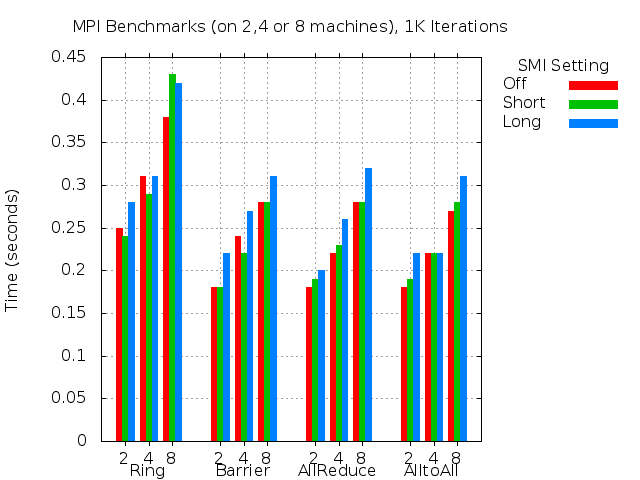
\includegraphics[keepaspectratio=true,width=240pt]{ss_graph1.png}
  \caption[cap1]{Multi-machine communication, 1K iterations, SMIs enabled on smitest3 only}
  \label{ss_graph1}
  \end{figure}
  & 
  \begin{figure}[H]
  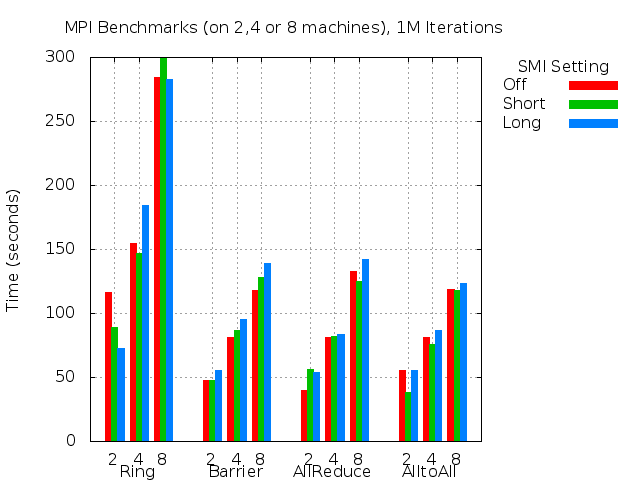
\includegraphics[keepaspectratio=true,width=240pt]{ss_graph2.png}
  \caption[cap2]{Multi-machine communication, 1M iterations, SMIs enabled on smitest3 only}
  \label{ss_graph2}
  \end{figure}\\
  \hline


  \begin{figure}[H]
  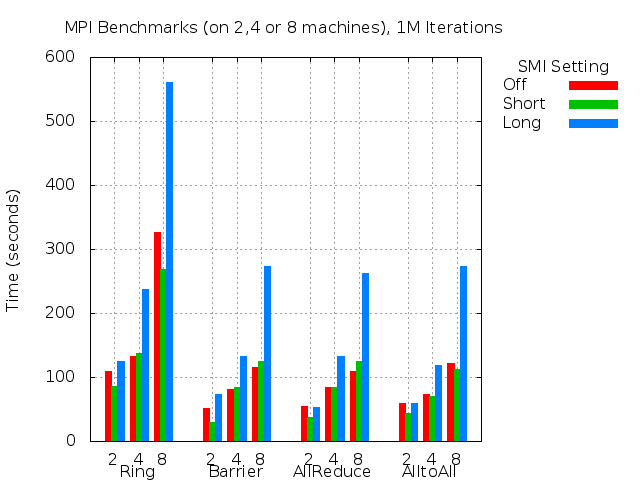
\includegraphics[keepaspectratio=true,width=240pt]{ss_graph3.png}
  \caption[cap3]{Multi-machine communication, 1M iterations, SMIs enabled on all smitest’s}
  \label{ss_graph3}
  \end{figure}
  & 
  \begin{figure}[H]
  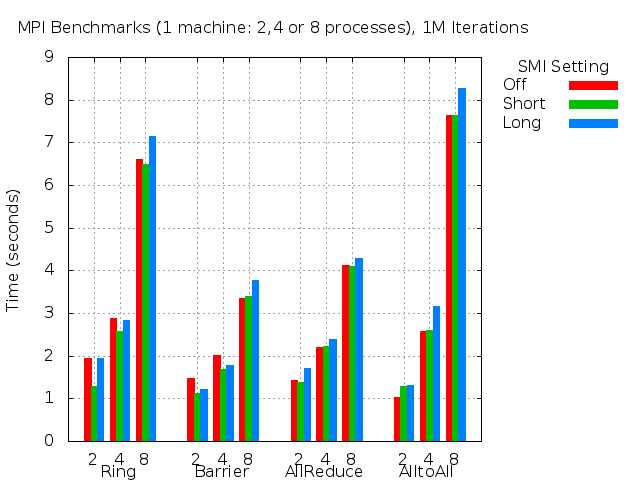
\includegraphics[keepaspectratio=true,width=240pt]{ss_graph4.png}
  \caption[cap4]{1 machine communication only, 1M iterations, SMIs enabled on smitest3}
  \label{ss_graph4}
  \end{figure}\\
  \hline
\end{tabular}
\end{table*}

Runtimes were obtained for tests upon only one machine, but with multiple processes, specifically using 2, 4, or 8 processes. This was done in order to possibly gain insight into whether SMIs affect performance of a multi-core machine. Originally, trials were attempted with only 1,000 iterations (graphed results are not provided). Although run times averaged longer than times obtained for the same tests ran upon multiple machines (averaging 1 second for almost all runs versus 0.2 to 0.4 seconds for multi-machine runs), the variance for these runs was quite drastic with run times of around 0.4 or 0.7 seconds periodically occurring amidst the same runs of around 1 second duration; even in the case of AllReduce with 2 processes (short SMIs enabled), all 3 trials were 0.05 seconds. When these aberrations were removed most runs showed very slight differences between enabling SMIs and not.

Thus, the same measurements were ran with iterations of 1,000,000 as is shown in Figure~\ref{ss_graph4}. Normalized times gave 105\% for short SMI-enabled runs and 94\% for long SMI-enabled runs. Significant differences were not observed between normalized times for 2, 4, and 8 processes, although 8 process runs tended to be slower by around 3\%. Long SMI runs tended to be around 90\% when considering the benchmark averages, except for Barrier which ran faster than normal and averaged a very high 106\%.  

Further tests were conducted with the one computer/multiple process set-up and are shown in Table~\ref{ss_table2}. These runs were only performed for the AlltoAll benchmark. Times were analyzed simply in comparison with times with no SMIs enabled (in the columns "\% Normalized Time), and times were incorporated with SMI counts to calculate "\% Remaining CPU clocks" in the same fashion as done in \cite{KD}. Upon learning that SMI latencies may not be consistent for smitest3 versus all other smitest machines (later discovered to be due to the hyperthreading setting enabled for smitest3 only), as explained in Section~\ref{sub:km_smilength}, similar tests were conducted upon smitest5. Two prominent features are evident. First, 2 process runs average less than half the time on smitest5 (although an occasional run did yield around 1.5 seconds with one SMI occurring on this machine). This leads to the difference in \% remaining CPU clocks. Second, there is a drastic difference in run times with 8 processes; additionally the \% normalized time varies largely for this run, with 93\% for smitest3 and 76\% for smitest5 although \% remaining CPU clocks are nearly identical. Thus, it appears that the use of hyperthreading allows for the runs with process number greater than number of cores to finish faster and to finish within similar time (only 8\% longer) to a run with no SMIs enabled. 

% Please add the following required packages to your document preamble:
% \usepackage[table,xcdraw]{xcolor}
% If you use beamer only pass "xcolor=table" option, i.e. \documentclass[xcolor=table]{beamer}
\begin{table*}
\caption{Comparison Between Machines with and without Hyperthreading Enabled}
\label{ss_table2}
\begin{adjustbox}{width=\textwidth,totalheight=\textheight, keepaspectratio}
\begin{tabular}{|l|l|l|l|l|l|l|l|l|l|}
\hline
\rowcolor[HTML]{FFFFFF} 
\cellcolor[HTML]{FFCCC9}All to All Benchmark & & \cellcolor[HTML]{FFFFC7}\begin{tabular}[c]{@{}l@{}}smitest3 (hyper-\\ threading)\end{tabular} & & {\color[HTML]{333333}} & & \cellcolor[HTML]{FFCE93}smitest5 (no hyper-threading) & & &\\
\hline
\rowcolor[HTML]{FFFFFF}
SMI Type & \# Processes & Average Time (seconds) & Average SMI Count & {\color[HTML]{333333} \% Remaining CPU clocks} & \% Normalized Time & \begin{tabular}[c]{@{}l@{}}Average\\ Time\\ (seconds)\end{tabular} & \begin{tabular}[c]{@{}l@{}}Average\\ SMI \\ Count\end{tabular} & \% Remaining CPU clocks & \% Normalized Time\\
\hline
\rowcolor[HTML]{FFFFC7}
Short & \cellcolor[HTML]{FFFFFF}2 & 1.59 & 1 & {\color[HTML]{333333} 100.0} & 99.6 & \cellcolor[HTML]{FFCE93}0.60 & \cellcolor[HTML]{FFCE93}0 & \cellcolor[HTML]{FFCE93}100.0 & \cellcolor[HTML]{FFCE93}94.5\\
\hline
\cellcolor[HTML]{FFFFFF} & \cellcolor[HTML]{FFFFFF}4 & \cellcolor[HTML]{FFFFC7}2.93 & \cellcolor[HTML]{FFFFC7}3 & \cellcolor[HTML]{FFFFC7}{\color[HTML]{333333} 100.0} & \cellcolor[HTML]{FFFFC7}100.3 & \cellcolor[HTML]{FFCE93}3.65 & \cellcolor[HTML]{FFCE93}3 & \cellcolor[HTML]{FFCE93}100.0 & \cellcolor[HTML]{FFCE93}101.3\\
\hline
\cellcolor[HTML]{FFFFFF} & \cellcolor[HTML]{FFFFFF}8 & \cellcolor[HTML]{FFFFC7}7.58& \cellcolor[HTML]{FFFFC7}7 & \cellcolor[HTML]{FFFFC7}{\color[HTML]{333333} 100.0} & \cellcolor[HTML]{FFFFC7}100.3 & \cellcolor[HTML]{FFCE93}40.97  & \cellcolor[HTML]{FFCE93}42 & \cellcolor[HTML]{FFCE93}100.0 & \cellcolor[HTML]{FFCE93}100.0  \\ 
\hline
\rowcolor[HTML]{FFFE65} 
Long  & \cellcolor[HTML]{FFFFFF}2 & 1.63& 1 & {\color[HTML]{333333} 93.3}  & 97.2  & \cellcolor[HTML]{FE996B}0.58& \cellcolor[HTML]{FE996B}0  & \cellcolor[HTML]{FE996B}100.0 & \cellcolor[HTML]{FE996B}97.1\\ 
\hline
\cellcolor[HTML]{FFFFFF}& \cellcolor[HTML]{FFFFFF}4 & \cellcolor[HTML]{FFFE65}3.16& \cellcolor[HTML]{FFFE65}3 & \cellcolor[HTML]{FFFE65}{\color[HTML]{333333} 89.6}  & \cellcolor[HTML]{FFFE65}93.0  & \cellcolor[HTML]{FE996B}3.86& \cellcolor[HTML]{FE996B}3  & \cellcolor[HTML]{FE996B}92.2  & \cellcolor[HTML]{FE996B}95.6\\ 
\hline
\cellcolor[HTML]{FFFFFF}& \cellcolor[HTML]{FFFFFF}8 & \cellcolor[HTML]{FFFE65}8.20& \cellcolor[HTML]{FFFE65}7 & \cellcolor[HTML]{FFFE65}{\color[HTML]{333333} 90.6}  & \cellcolor[HTML]{FFFE65}92.6  & \cellcolor[HTML]{FE996B}54.15  & \cellcolor[HTML]{FE996B}51 & \cellcolor[HTML]{FE996B}90.5  & \cellcolor[HTML]{FE996B}{\color[HTML]{FE0000} 75.7} \\ 
\hline
\end{tabular}
\end{adjustbox}
\end{table*}

\textbf{Conclusion and Future Work}

Tests with MPI programs, although not thoroughly conclusive, do provide some additional insight into the effects of SMIs upon parallel, communicating computers in a cluster. The most prominent conclusion is that long (~100 ms) SMIs incur an additive penalty upon performance. For the benchmarks tested with long SMIs enabled upon all machines, the ratio between time with long SMIs enabled versus no SMIs enabled can be as much as 2.5 times longer, with 8 node communication. Less dramatic effects are witnessed when SMIs are enabled upon only 1 machine of the cluster, nevertheless a performance penalty is still incurred; such penalties are relative to single core, single machine benchmarks, usually matching the latency of the SMI. Another observation is that short SMI runs sometimes produce faster run times, which is not easily explainable; perhaps some change in normal scheduling occurs because of these interrupts or the accounting of time is incorrect. Hyperthreading is another variable that may be a factor to possibly ameliorate the effects of long SMIs upon a run.

For future work, all tests should be performed again because all tests except that using smitest5 in Table\ref{ss_table2} were performed using smitest3, and smitest3 had hyperthreading enabled. Also, more trials need to be performed in order to reduce variance. Further testing can be performed with the enabling of hyperthreading to ascertain its effect in relation to SMI enabling. Possible synchronization of SMI timing may be an interesting test to determine this parameter upon MPI benchmarks possibly akin to studies in reducing noise in high performance computation 
%\{P. Beckman, K. Iskra, K. Yoshii, S. Coghlan, and A. Nataraj,
%“Benchmarking the effects of operating system interference on extreme-scale parallel machines,” Cluster Computing 11(1): pp. 3-16, 2008.\} 
\emph{\cite{NHPC}}. Lastly, other benchmarks can be tested, such as NAS (NASA MPI) benchmarks or other prominent MPI benchmarks. Especially, the tests in this paper mainly tested the MPI routines, thus MPI communication was particularly tested. It may be interesting to incorporate more computation into the mix or other important features like memory use and disk reads.

%\begin{table*}
%\caption{MPI Benchmark Tests}
%\label{ss_table2}
%\vspace*{0in}
%\begin{adjustbox}{width=\textwidth,totalheight=\textheight, keepaspectratio}
%  \begin{tabular}{|l|l|
%      >{\columncolor[HTML]{FFFC9E}}l|l|
%      >{\columncolor[HTML]{FFFC9E}}l|l|}
%      \hline
%      All to All Benchmark & & {\color[HTML]{333333} smitest 3 (hyperthreading)} &  & \begin{tabular}[c]{@{}l@{}}smitest 5 \\ (no hyperthreading)\end{tabular} &  \\ \hline
%      SMI Type & \# Processes & {\color[HTML]{333333} \% Remaining CPU clocks} & \% Normalized Time & \% Remaining CPU clocks & \% Normalized Time \\ \hline
%      Short & 2 & {\color[HTML]{333333} 100.0} & 99.6 & 100.0 & 94.5 \\ \hline
%     & 4 & {\color[HTML]{333333} 100.0} & 100.3 & 100.0 & 101.3 \\ \hline
%    & 8 & {\color[HTML]{333333} 100.0} & 100.3 & 100.0 & 100.0 \\ \hline
%   &  & {\color[HTML]{333333} } &  &  &  \\ \hline
%   Long & 2 & {\color[HTML]{333333} 93.3} & 97.2 & 100.0 & 97.1 \\ \hline
%  & 4 & {\color[HTML]{333333} 89.6} & 93.0 & 92.2 & 95.6 \\ \hline
% & 8 & {\color[HTML]{333333} 90.6} & 92.6 & 90.5 & {\color[HTML]{FE0000} 75.7} \\ \hline
%\end{tabular}
%\end{adjustbox}
%\end{table*}

\subsection{Netperf}\label{sub:jm_netperf}
% =========================
% netperf begin
\textbf{Background}
The effects of SMM on networking are of particular interest because
SMIs may not only affect the local system but also all systems
connected to it.
Delgado and Karavanic investigated the effects
of SMM on TCP throughput and found that long SMIs reduce the throughput at a
scale directly related to the time spent in SMM while short SMIs may
not have any noticeable effect on throughput at all \cite{KD}.
We sought to confirm their results   
and to expand the investigation to UDP transmit.

To gain a better understanding on how adverse effects propagate between two hosts,
   we performed all tests twice, first with SMIs
   active on the server (sender) but not on the client (receiver), then with
   SMIs active only on the client side of the connection.
   In Figures~\ref{jm_graph1}, \ref{jm_graph2} and
   in Tables~\ref{tab:jm_tcp}, \ref{tab:jm_udp} we use the
   following notation to refer to these two
   cases: \textit{Sender(SMI) $\Rightarrow$ Receiver}
   and \textit{Sender $\Rightarrow$ Receiver (SMI)}.

   \textbf{Methodology}
   Netperf 2.6 \cite{NETPERF} was used to measure the throughput between two
   cluster nodes. Each type of test was performed for varying levels of SMIs, and
   multiple long SMIs were issued back to back to simulate longer SMIs.
   Each test ran for 60 seconds and was repeated five times; all reported
   numbers are the average of these five trials.

   \textbf{Results and Discussion}
   The effects of long SMIs on TCP throughput are shown in
   Figure~\ref{jm_graph1}. The leftmost bar in the chart indicates the
   remaining CPU time available to the system after subtracting the amount
   of time spent in SMM. The middle bar shows the throughput for the case
   where SMIs are enabled only on the server. The right bar shows the
   throughput for the case where SMIs are enabled only on the client. Our
   results confirm that the drop in throughput scales with the amount of
   time spent in SMM. The results also show that in cases where SMIs are
   enabled on the client but not on the server, the client experiences some
   additional degradation due to overhead in the form of TCP packet
   retransmissions.
   Table~\ref{tab:jm_tcp} illustrates this effect further.

   Table~\ref{tab:jm_tcp} shows the amount of data that was transferred between two
   hosts in 60 seconds and the average number of TCP retransmissions, which is virtually
   zero in the case where the client was not interrupted by SMIs (top rows).
   This changes if the client is slowed down by SMIs (bottom rows).
   For example, with one long SMI per second, almost 50,000 retransmissions
   (800 / sec) occurred. Interestingly, this number decreases with increasing
   amount of time spent in SMM. For instance, with five long SMIs per second,
   only half the number of retransmissions occurred. The inherently lower
   transfer rate at that point explains this phenomenon.

   The effects of long SMIs on UDP throughput are shown in Figure~\ref{jm_graph2}.
   Most importantly, we did not see a significant difference between
   TCP and UDP in terms of their sensitivity to SMM.
   Like TCP, the drop in throughput scales with the amount of time spent
   in SMM.  
   Unlike TCP, both cases (SMIs enabled on the sender but not on the receiver,
   and vice versa) experienced the same level
   of degradation, which was to be expected since UDP is a stateless protocol.
   However, the reasons for the drop in throughput are different. If the server
   is slowed down by SMIs, then the drop in throughput is just a consequence
   of the server sending at a lower rate.  If the client is slowed down by SMIs,
   then the drop in throughput is caused by the receiver being unable to process
   all incoming UDP datagrams. So while the throughput between the two cases
   is the same, the amount of data sent over the network is not. This is
   further detailed in Table~\ref{tab:jm_udp}, which shows the results
   for the 60 second UDP transmits in terms of the amount of
   data (in gigabytes) the server sent and the amount of data the client received.

   To determine the effect of short SMIs, throughput was measured for the
   following five different scheduling intervals:  1, 10, 100, and 500 short
   SMIs per second. All the individual benchmarks experienced no throughput
   degradations, neither for TCP nor UDP. Hence, our results are identical
   to the findings reported by Delgado and Karavanic, who explain their results
   arguing that "SMI usages that are able to interleave SMIs with I/O may
   be able to avoid the full penalty of the SMI." \cite{KD} We concur.

   \textbf{Conclusion and Future Work}
   Our results show that long SMIs can have a significant effect on network
   throughput. More specifically, the performance penalty is closely linked
   to the length of the amount of time spent in SMM.
   Systems at the receiving end of a data connection that are frequently
   interrupted by long SMIs may experience some additional degradation
   if they fail to keep up with the incoming data stream to an extent to which
   the server starts to retransmit data.
   Additional traffic ultimately affects all systems on the network.
   By contrast, short SMIs seem to have no significant effect on network throughput.
   
   Netperf can also be used to measure CPU utilization and latency. All future work
   should include these two important aspects of network performance.

   \begin{figure}[H]
   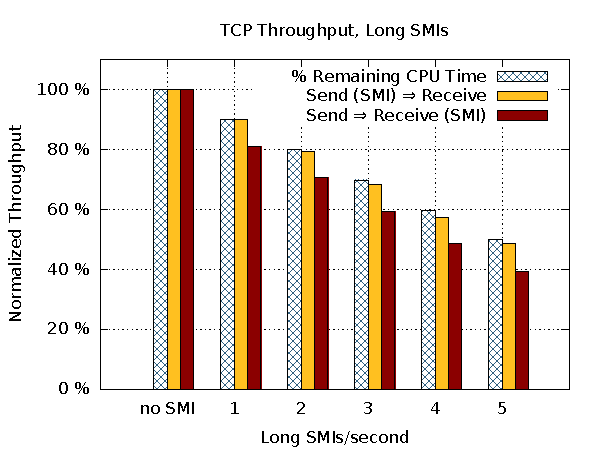
\includegraphics[keepaspectratio=true,width=240pt]{jm_graph1.pdf}
   \caption{TCP throughput scaled against a baseline for varying levels of SMIs;
       Maximum Std. Deviation 1.5\%}
       \label{jm_graph1}
       \end{figure}
       %---------------
       % ``specialcell'' is to force a linebreak in table cell; found this here:
       % http://tex.stackexchange.com/questions/2441/how-to-add-a-forced-line-break-inside-a-table-cell
       \newcommand{\specialcell}[2][c]{%
             \begin{tabular}[#1]{@{}c@{}}#2\end{tabular}}
             % ---------------  
             \begin{table}[h]
                               \caption{60 sec TCP Data Transfer, Long SMIs; Max Std-Dev is 102 MB}
                               \label{tab:jm_tcp}
             \centering
             \begin{tabular}{c|c|c}
             \textbf{\specialcell{\# SMIs /\\Second}}
             & \textbf{\specialcell{GB Transferred via TCP\\Send (SMI) $\Rightarrow$ Recv}}
             & \textbf{\# Retransmissions} \\
                 \hline
                 0 & 5.60 & 0 \\
                     1 & 5.05 & 0 \\
                     2 & 4.43 & 0 \\
                     3 & 3.82 & 3 \\
                     4 & 3.21 & 2 \\
                     5 & 2.71 & 7 \\
                       &    & \vspace*{12px}\\   %%% some spave between two tables
                       \textbf{\specialcell{\# SMIs /\\Second}}
                       & \textbf{\specialcell{GB Transferred via TCP\\Send $\Rightarrow$ Recv (SMI)}}
                       & \textbf{\# Retransmissions} \\
                           \hline
                           0 & 5.60 & 0 \\
                               1 & 4.53 & 49865 \\
                               2 & 3.95 & 45418 \\
                               3 & 3.32 & 37518 \\
                               4 & 2.71 & 28775 \\
                               5 & 2.20 & 24722 \\
                               \end{tabular}
                               \end{table}
                               % --------------

                               \begin{figure}[H]
                               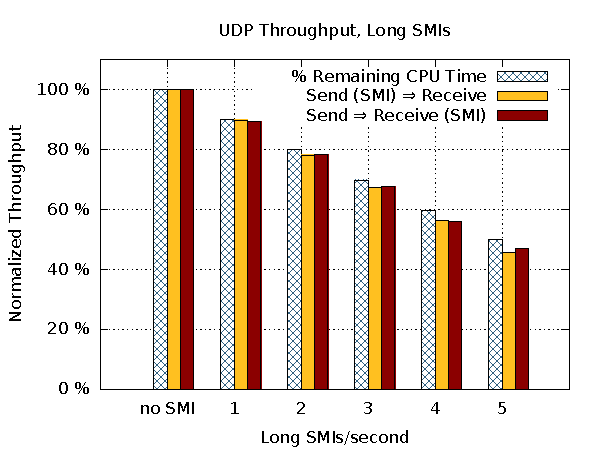
\includegraphics[keepaspectratio=true,width=240pt]{jm_graph2.pdf}
                               \caption{UDP throughput scaled against a baseline for varying levels of SMIs;
                                   Maximum Std. Deviation 1.2\%}
                                   \label{jm_graph2}   
                                   \end{figure}
                                   % ---------------



                                   \begin{table}[h]
                                           \caption{UDP Data Transfer, Long SMIs; GB Sent and GB Received in 60 sec; Max
                                               Std-Dev is 102 MB}
                                               \label{tab:jm_udp}
                                   \centering
                                   \begin{tabular}{c|c|c}
                                   \textbf{\specialcell{\# SMIs /\\Second}}
                                   & \textbf{\specialcell{GB Transferred via UDP\\Send (SMI) $\Rightarrow$ Recv}}
                                   & \textbf{\specialcell{GB Transferred via UDP\\Send $\Rightarrow$ Recv (SMI)}} \\
                                       \hline
                                       0 & 5.71 $\Rightarrow$ 5.71 & 5.71 $\Rightarrow$ 5.71 \\
                                           1 & 5.13 $\Rightarrow$ 5.13 & 5.71 $\Rightarrow$ 5.09 \\
                                           2 & 4.46 $\Rightarrow$ 4.46 & 5.71 $\Rightarrow$ 4.48 \\
                                           3 & 3.84 $\Rightarrow$ 3.84 & 5.71 $\Rightarrow$ 3.86 \\
                                           4 & 3.22 $\Rightarrow$ 3.22 & 5.71 $\Rightarrow$ 3.19 \\
                                           5 & 2.60 $\Rightarrow$ 2.60 & 5.71 $\Rightarrow$ 2.68 \\
                                           \end{tabular}
                                               \end{table}
                                               %netperf end
                                               %===========



\subsection{LMBench}\label{sub:lmbench}

\textbf{Background}
Lmbench is a tool for performance analysis for applications. Application tasks are divided into threads and then executed as individual units but these threads may or may not be dependent upon each other for input or data. For data passing, they need to communicate, and how much time they spend to establish connections and transfer data will directly affect performance. Lmbench is a simple suite of portable benchmarks which run a number of benchmarks such as ones which test bandwidth, latency, and system call overhead for different file sizes and memory sizes. Lmbench provides a suite of benchmarks that attempt to measure the most commonly found performance bottlenecks in a range of applications by measuring overhead in interprocess communication, data transfer rate and context switching \cite{LMB}.\\

\textbf{Methodology}
Lmbench provides many bandwidth and latency benchmarks, therefore we will only analyze a few of them to determine the effect of SMIs on application performance. The LMbench tool runs applications by dividing them into several threads and then checks the time to establish connection between processes. In the User Data Protocol (UDP), no acknowledgement of data transfer occurs. Performance is measured by finding UDP latency. If UDP latency between two processes is prolonged upon enabling of SMIs, this indicates that the SMIs are increasing communication time, indicating that they are directly adding time for application execution. In contrast to UDP, the Transmission Control Protocol (TCP) provides acknowledgement for connection establishment between processes. A comparison is also made for TCP latency when SMIs are enabled with short and long durations and when they are not enabled. Additionally, pipe bandwidth, which is where output of one process is transferred to another process as input, is measured in Lmbench. Lastly, the time difference for creation, termination and execution of processes is measured in comparison to SMI enabling. 

\textbf{Results and Discussion}
UDP latency, TCP latency, and TCP and UDP latency for Remote Procedure Call (RPC) with short SMIs yield run times of almost same amount as runs with no SMIs enabled, showing very little difference. There is considerable difference between these latencies when duration of SMIs is increased (when long SMIs are enabled). We can see results in Graph \ref{mb_graph1.png} that there is quite a large difference even between short SMI and no SMI for times taken to establish TCP/IP connection.\\

%GRAPH GOES HERE
\begin{figure}[H]
   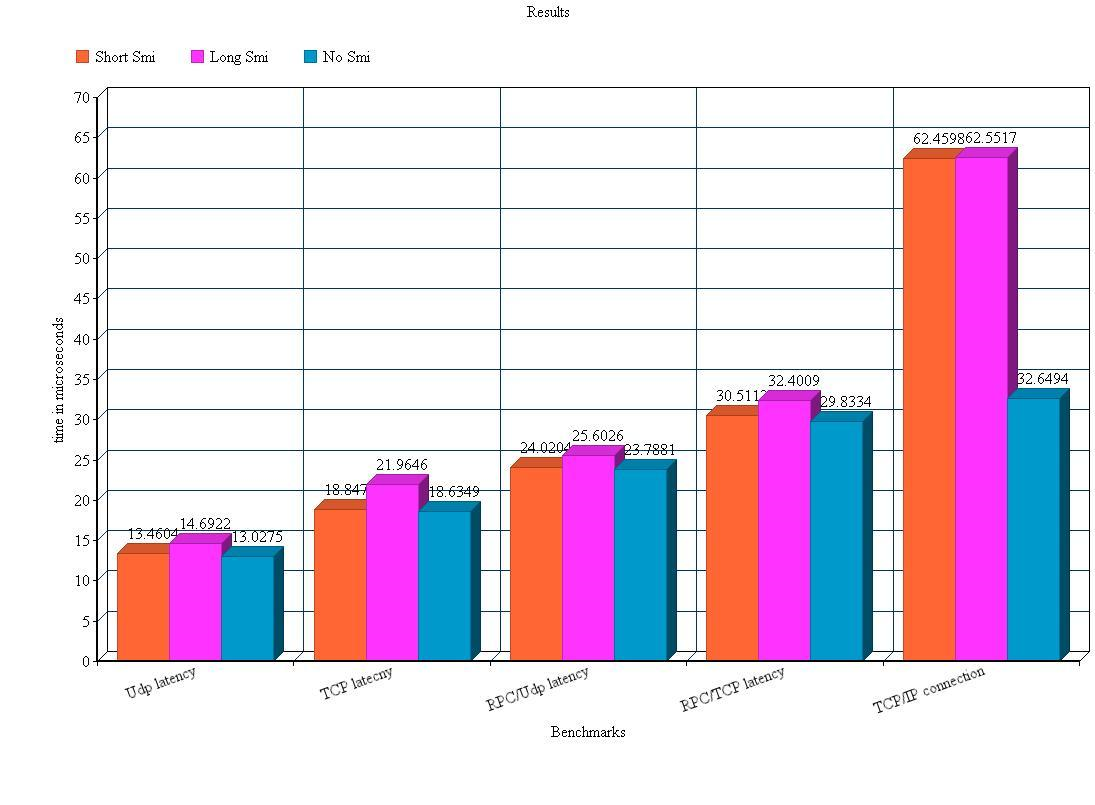
\includegraphics[keepaspectratio=true,width=240pt]{mb_graph1.png}
   \caption{ }
\end{figure}

We also measured the rate of data transfer when output of one process acts as input to another process. We can see the results listed below. The bandwidth is maximum when SMIs are disabled. Only a 13 Mb/sec difference exists when short SMIs are enabled but a difference of 233 Mb/sec occurs when long SMIs are enabled.\\

%%%%%%%%%%%%%%%%%%%%Table here
\begin{table}[H]
\caption{ }
\centering
\begin{tabular}{|c|c|c|}
  \hline
  Short SMI & Long SMI & No SMI\\
  \hline
  1970 Mb/sec & 1750 Mb/sec & 1983 Mb/sec\\
  \hline
\end{tabular}
\end{table}

Below, the results for time in creating a process and terminating it are displayed. Also is shown the time for creating a process and executing it, as well as for creating a process and executing it in system shell. In these, little difference exists between times of runs with short SMIs and runs with no SMIs, but there is considerable difference when long SMIs are enabled.\\

%ANOTHER GRAPH HERE
\begin{figure}[H]
   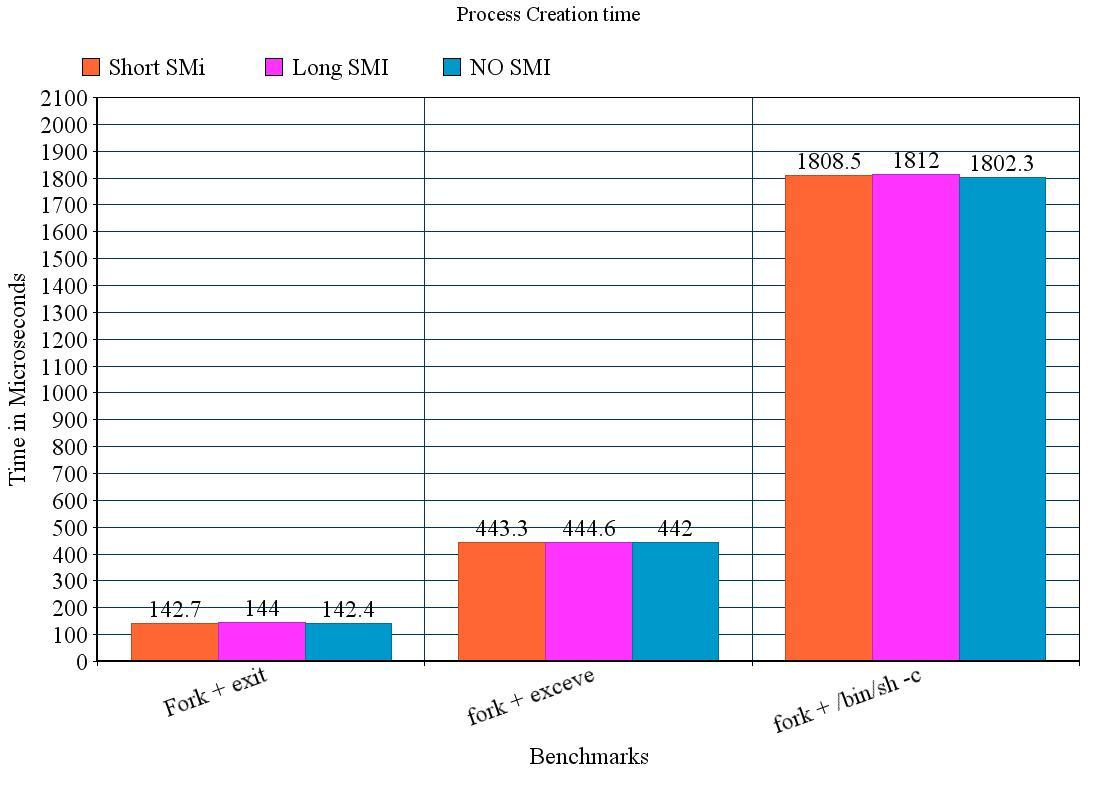
\includegraphics[keepaspectratio=true,width=240pt]{mb_graph2.png}
   \caption{ }
\end{figure}

\textbf{Conclusion and Future Work}
After running Lmbench tool on the provided machines, the results clearly indicate that SMIs are not a bottleneck to performance when their durations are short, but they are when the duration of SMIs is increased. There is very small difference in performance of applications when short SMIs are enabled and SMIs are disabled, so future work would be to find SMI duration where application performance is the exactly same as when SMIs are disabled. This would serve the purpose of protecting system from issues like power throttling without any performance overhead.\\

\subsection{NBench}\label{sub:nbench}
\textbf{Background}
The Nbench benchmark measures the performance of the computation power of the CPU by calculating integer computation index, floating point index and memory access 
index (combined sequential and non sequential memory access). Its measurement can give an idea of how well a system will perform. It runs a set of C programs to calculate the performance measurement indices. Nbench uses the runtime statistics to calculate the indices. The set of programs are divided into two major sets: 1) Integer computation and memory access and 2) Floating point computations. The test suite consists of the following set of programs.

\textbf{1. Integer Computation and Memory Access}
\begin{itemize}
\item Numeric Sort - Sort an array of 32 bit integers
\item String  Sort - Sort an array of strings of arbitrary lengths
\item Assignment - Task allocation algorithm
\item Idea Encryption - Block cipher encryption algorithm  
\item Huffman - Text and Graphics compression algorithm 
\end{itemize}
\textbf{2. Floating-point Computation}
\begin{itemize}
\item Fourier Coefficients - Series approximation of waveforms 
\item Lu Decomposition - Algorithm for solving linear equations  
\item Neural Net - Functional back-propagation network simulator
\end{itemize}

\textbf{Methodology}
The Nbench test suite is based upon dynamic workload. It performs timing using a stopwatch paradigm. The method StartStopwatch() begins timing, and StopStopwatch() ends timing and reports the elapsed time in clock ticks. The benchmark has a global variable called GLOBALMINTICKS. This variable is the minimum number of clock ticks that the benchmark runs for a particular program. It only allows this minimum clock ticks to report to StopStopwatch(). For example, if one runs numeric sort, the program will construct an array filled with random numbers, call the StartStopwatch(), sort the array and then call StopStopwatch(). If the reported time in StopStopwatch() is less than GLOBALMINTICKS, the benchmark will build two arrays and will try again to sort them. The process is repeated until the StopStopwatch() routine reports the minimum time ticks, being GLOBALMINTICKS. This principle is applied to all the tests in the benchmark.\cite{TUX}

\textbf{Results and Discussions}
All the tests were ran for 10 trials upon the same machine (smitest2), and the average was obtained for these trials. During benchmark runs, it was verified that no other process ran in the system to avoid affecting the running time computation of the benchmark. 

For both short and long SMI's the average iterations/sec were affected and reduced. For example, for numeric sort the average iterations/sec were reduced from 1172 to 1123 and 1079, for short and long SMI runs, respectively. For long SMIs, similar behavior was observed for the rest of the programs for integer computation and memory access. However there were anomalous results for the short SMI case. In 4 out of 10 runs, the iterations/sec increased slightly for all the programs of this category. The following graph depicts this behavior for all the programs in integer computation and memory access. 

%%%%%%%%%GRAPH1 GOES HERE
\begin{figure}[H]
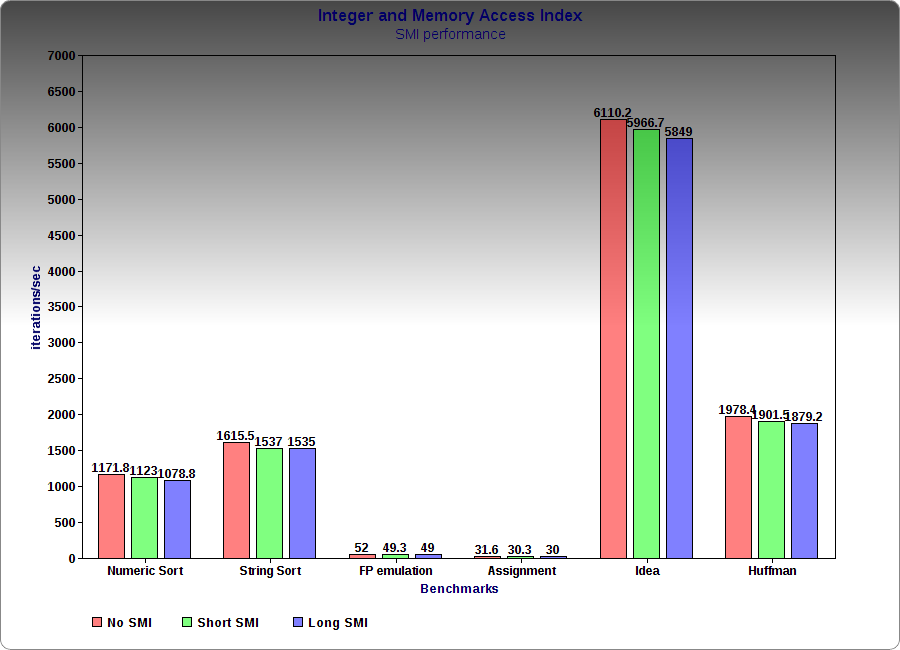
\includegraphics[keepaspectratio=true,width=240pt]{vj_graph1.png}
\caption{ }
\end{figure}

Similar behavior occurred for floating-point computation programs. Four out of 10 test runs showed performance improvement in short SMI runs, whereas long SMIs always degraded the computation capacity of the programs. The following graph depicts this behavior.

\begin{figure}[H]
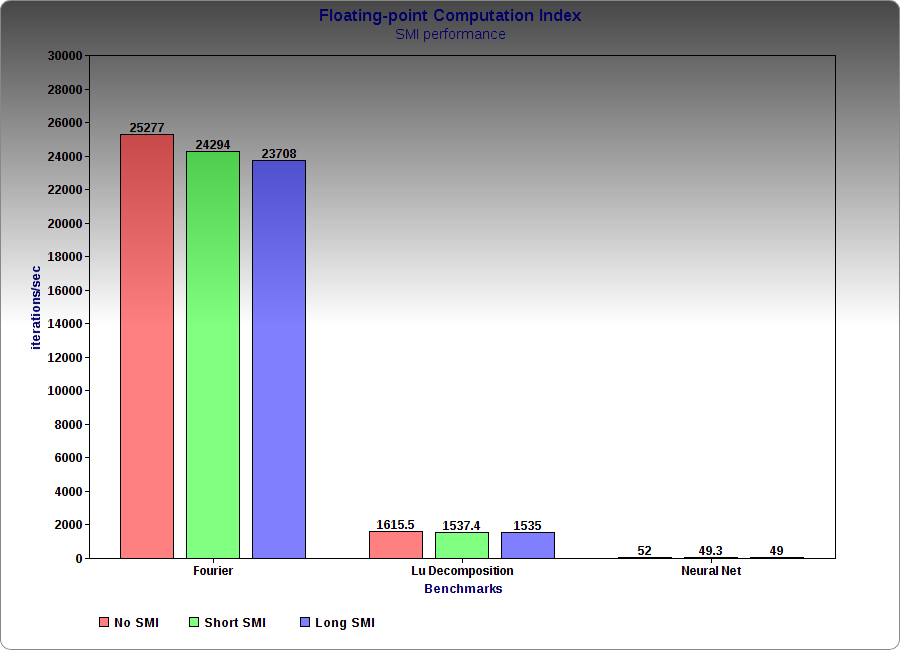
\includegraphics[keepaspectratio=true,width=240pt]{vj_graph2.png}
\caption{ }
\end{figure}

%%%%%%%%%GRAPH2 GOES HERE


The main idea of the Nbench benchmark is to generate a set of indices which reflect the overall performance of the system. In this benchmark, we get an index score for integer     computations, memory access and floating-point computations. Three set of index scores were calculated to measure the performance of the system in no SMI mode, short SMI mode and long SMI mode. The following graph shows that as an average of 10 runs the index score is less for both short SMI and long SMI. However the change in short SMI mode is comparatively less in short SMI than in long SMI.

\begin{figure}[H]
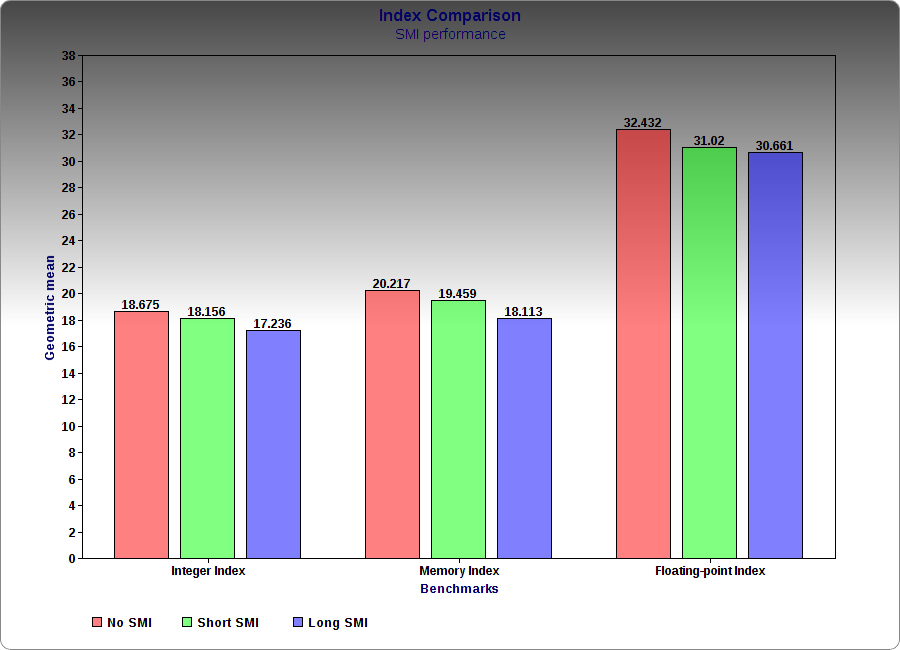
\includegraphics[keepaspectratio=true,width=240pt]{vj_graph3.png}
\caption{ }
\end{figure}
%%%%%%%%%GRAPH3 GOES HERE

The percent change for these indices in given in the following table.

\begin{table}[h]
            \caption{ }
\begin{tabular}{lll}
\hline
Index                      & Short SMI & Long SMI \\ \hline
Integer Computation        & 2.7       & 7.7      \\
            Memory Access              & 3.7       & 10.4     \\
            Floating-point Computation & 4.3       & 5.4      \\ \hline
            \end{tabular}
            \end{table}


\textbf{Conclusion and Future Work}
The results of the Nbench benchmark clearly indicate that SMIs interrupt the execution of the application computation. It affects the running time and iterations/sec for all of the test suite program. Long SMIs greatly affects the system performance and care should be taken to ensure that the system spends the least possible time in System Management Mode. Short SMIs do not significantly affect the running time of the application computation. For a noticeable number of cases the iterations/sec were increased slightly for all the programs of the test suite. The performance degradation was only visible when calculating the average of 10 runs. For the future work, especially to arrive at a definite conclusion for benchmark runs with short SMIs, a larger trial set size should be used. Investigation should be done to definitively determine the length of the SMIs, and their performance impact should be studied separately so that a clear definition for long SMI and short SMi can be established. Finally, these Nbench benchmarks should be run in a multiprocess environment where each process is doing some meaningful work. Performance impact of SMIs in such cases should be studied to understand its impact.
\subsection{Power}\label{sub:power}
\textbf{Background}
An ever present performance concern, power continues to be an issue for developing technologies, including those 
revolving around the SMM abstraction layer. New tools such as HyperSentry \cite{HYPSENT} and Hypercheck \cite{HYPCH}
execute runtime checks on hypervisors by way of SMM. Depending on the length frequency of these checks systems may encounter significant power drains to which underlying abstraction layers may be completely unaware of. 

\textbf{Methodology}
CPU power states were measured using Turbostat, a tool for gathering data on the time spent 
in various CPU power states. While running, Turbostat reports on an interval the 
percentage time spent in power states $C\_0$ ( Full power), $C\_1$, $C\_3$, and $C\_6$ (deepest sleep state). 
A control report was first created by running Turbostat on an idle machine for 5 minutes. 
While never completely idle, Turbostat reported that the majority of time was spent in $C\_0$. Next, Turbostat was run with a stream of short (~0.05ms) SMI’s occurring every second for 5 minutes. Lastly, Turbostat was run with a stream of long ( ~100ms - 110ms) SMI’s occurring every second for 5 minutes.

\textbf{Results and Discussion}
While short SMI’s generated a relatively negligible effect on power consumption, 
long SMI’s produced significant reductions in percentage time spent in deep sleep states. 
While running long SMI’s, Turbostat reported almost a 25\% decrease in time spent in $C\_6$, the deepest CPU sleep state.
In addition, CPU states $C\_0$ and $C\_3$ both saw an increase of about 10\% 
in percentage time spent in the states as illustrated in fig. bellow. 
While programs such as HyperSentry and HyperCheck only generate 35ms SMI’s, 
clearly sustained SMI generation has the potential to cause significant reductions in power efficiency.
\begin{figure}[H]
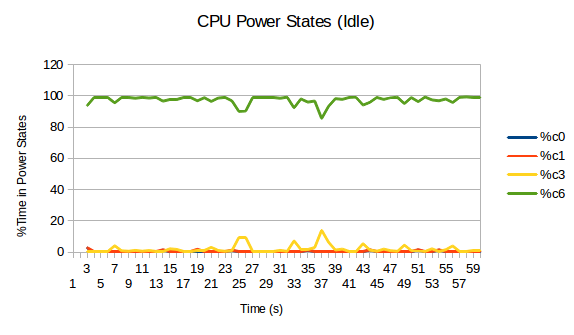
\includegraphics[keepaspectratio=true,width=240pt]{wh_idle.png}
\caption{ }
\end{figure}
\begin{figure}[H]
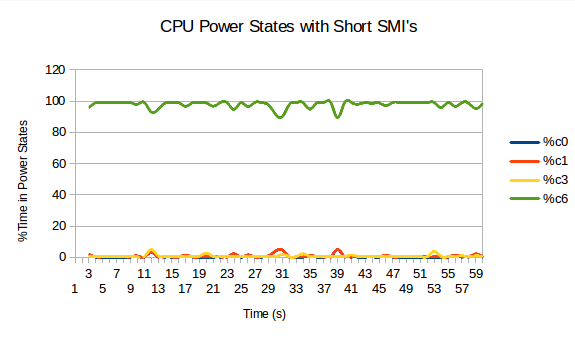
\includegraphics[keepaspectratio=true,width=240pt]{wh_short.png}
\caption{ }
\end{figure}
\begin{figure}[H]
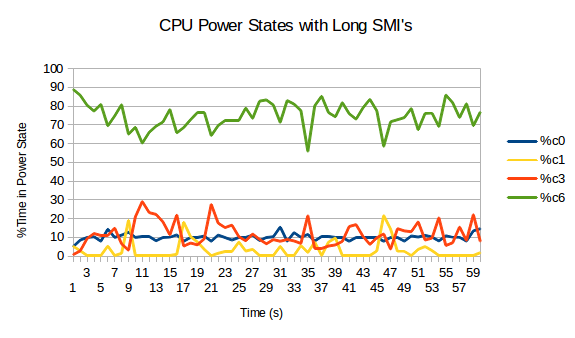
\includegraphics[keepaspectratio=true,width=240pt]{wh_long.png}
\caption{ }
\end{figure}
\textbf{Conclusion}
Short SMIs do not seem to change power states from that produced when no SMIs are used. In contrast, when long SMIs are enabled, much more time is spent in higher powered states.
This matches observation of Delgado and Karavanic.

\section{General Conclusion}
In this work, we investigated the effects of SMIs on system performance and power management. The used benchmarks, which included Linux kernel compilation, NBench, Netperf, LMBench, and custom built MPI benchmarks, allowed us to report on CPU bound computation, network throughput, network latency, memory access time, and MPI functions. We compared the effects of ``long'' (100 ms) and ``short'' (1 ms) SMIs against the baseline, and our results show that long duration SMIs may have a significant impact upon system performance. In fact, our findings reconfirm that performance degradation scales with the latency of the SMI. On the other hand, short SMIs seem to have no noticeable effect, particularly if they are interleaved with I/O. Long SMIs can be detrimental upon performance for multi-machine communication. Hyperthreading is an interesting parameter for measuring performance effects of SMIs. Short SMIs do not seem to change power states from that produced when no SMIs are used. In contrast, when long SMIs are enabled, much more time is spent in higher powered states.
This matches observation of Delgado and Karavanic.

\bibliographystyle{ieeetr}
\bibliography{bibliography}
\end{document}
